\documentclass[a4paper, 12pt]{article}
\usepackage{ctex} %使文档可以输入中文
\usepackage{amsfonts}
\usepackage{float}
\usepackage{graphicx}
\usepackage{amsmath,amssymb,amsfonts}
\begin{document}
	\title{黑洞渲染}
    \section{概述}
    电影星际穿越中的黑洞(卡冈图雅)给人留下了深刻的印象,此项目想对渲染其进行复现。
    \section{大致路线一}
    固定摄像机,用cpu渲染一张静态的(或许可以结合gpu渲染动态)黑洞照片。
    \subsection{非欧时空下的光线步进}
    一般渲染中的光线都是直线,但在黑洞周围时空高度扭曲,光线变成了时空上的测地线,
    需要用光线步进计算这条线。\\
    *目前已经用cpu实现了这一步,可视化如下:
    \begin{figure}[H]
        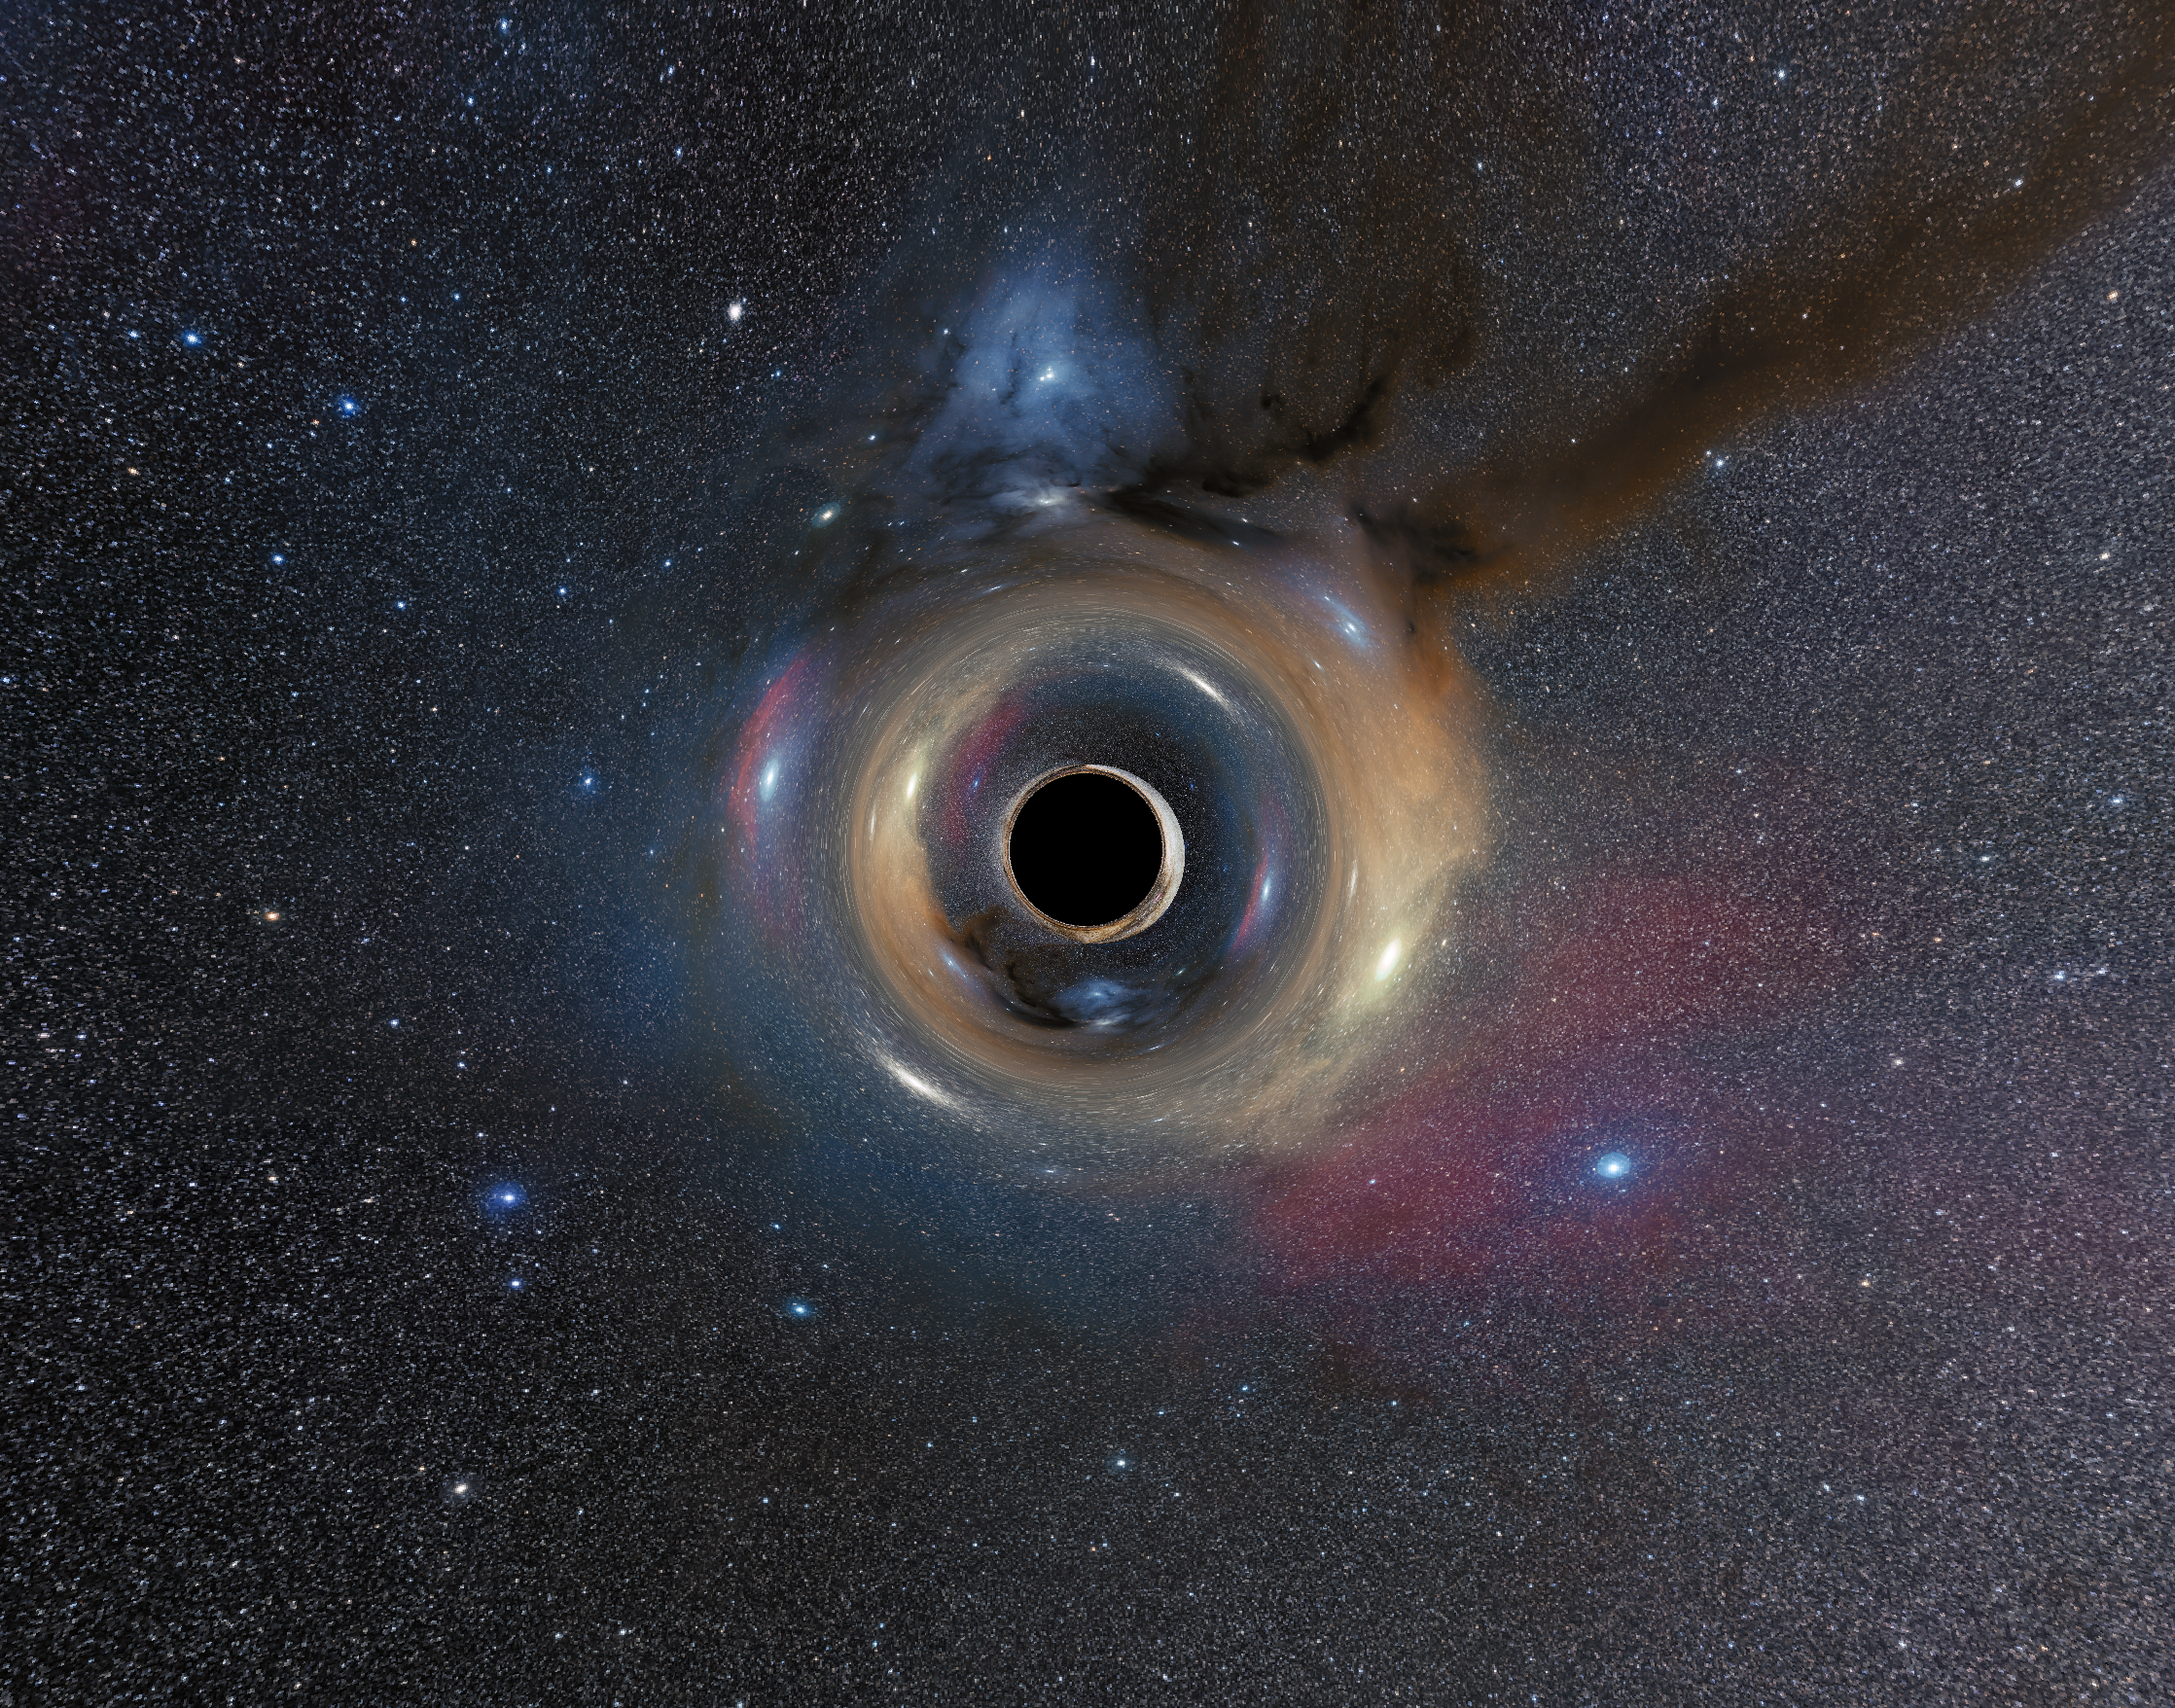
\includegraphics[width=1.0\textwidth]{1.png}
        \caption{无吸积盘的施瓦西黑洞(无旋转,不带电)} % 图片标题
    \end{figure}
    *这张图用的星空天空盒是直接拿一张png算的,导致有的地方颜色有突变,看起来黑洞边上有一团
    东西,但实际上程序中并没有设置任何物质,只是单纯的将星光射到摄像机。
    \subsection{体积渲染}
    为了计算吸积盘,需要用体积渲染计算光线的强度。可能需要一些采样技巧。\\
    测试:先拿平直时空下试(雾的密度可以设成氢原子轨道之类的函数,方便查看正确性)。\\
    \begin{figure}[H]
        \includegraphics[width=1.0\textwidth]{2.png}
        \caption{星际穿越里的一部分} % 图片标题
    \end{figure}
    *这个项目也有很多其他人做过,但似乎都是用一次采样(吸积盘设置为薄圆盘),我们也许可以做得更好,
    让吸积盘看上去有厚度。
    \subsection{物理更正}
    有如下需要修正的:
    1.光线的亮度/颜色如何受黑洞影响?\\
    2.考虑吸积盘的多普勒效应,一侧的吸积盘会偏暗偏红(星际穿越的导演觉得
    最终成图不好看,为了艺术性,将多普勒效应砍掉了。我想看看加上会如何。)
    \subsection{后处理}
    也许可以采用高斯模糊之类的手段提升视觉效果。
    \section{大致路线二}
    如果认为一的难度高,也可以将2.1用gpu重写。(cpu下实际渲染速度很慢,1080p可能每秒不超过
    10帧,尽管每个像素点的运算只是
    简单的两次矩阵乘法)

    
\end{document}